
\begin{frame}
\frametitle{What do we talk about when we talk about Spin?}
\begin{columns}
 
\column{0.5\textwidth}
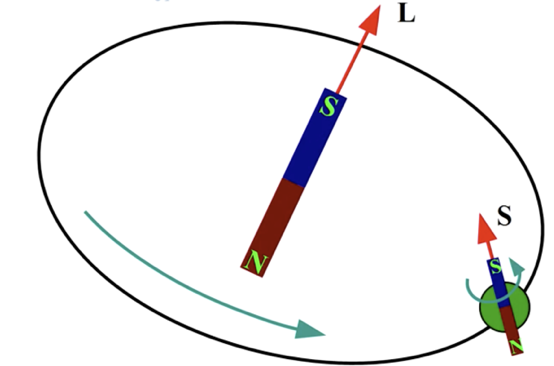
\includegraphics[scale=0.1]{img/electronMagnet.png}
The cartoon pictures the ``classical'' view of an atom (hydrogen), seen as a tiny magnet. The electron ``orbiting'' around the nucleus is said to have an (orbital) angular momentum defined by:
\[
\va{L} = \va{r} \times \va{p}
\]

From a classical perspective, as an electron carries a charge, its orbital motion will result in a tiny current loop which will produce a dipolar magnetic field. The strength of this dipole field is measured by the magnetic moment $\mu$ which is related to the orbital angular momentum by:
\[
\vv{\bm{\mu_L}} = \frac{q}{2m}\vv{\bm{L}} 
\]
\column{0.5\textwidth}
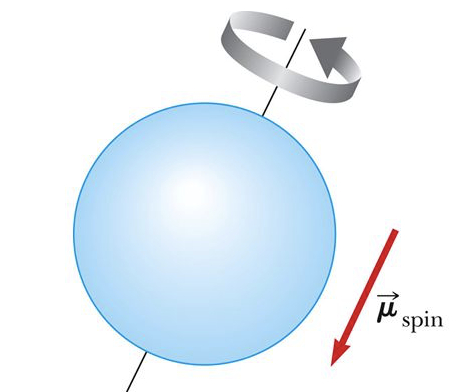
\includegraphics[scale=0.1]{img/classicalElectronSpin.png}
The classical idea of spin follows directly from the above considerations. Spin is the angular momentum we associate with a rotating sphere. If the sphere possesses an electric charge, then the circulation of the charge around the axis of rotation will constitute a current and hence will give rise to a magnetic field. This field is a dipole field whose strength, for a uniformly charged sphere of total charge q, is:

\[
\vv{\bm{\mu_L}} = \frac{q}{2m}\vv{\bm{S}} 
\]
\end{columns}
\end{frame}

\begin{frame}
\frametitle{Spin is a quantum effect}
 
The classical view of spin requires that the spinning sphere example has a non-zero radius. Classically a point particle can only have a spin angular momentum of zero and so it cannot have a magnetic moment. Thus, from the point-of-view of classical physics, elementary particles such as an electron, which are known to possess spin angular momentum, cannot be viewed as point objects -- they must be considered as tiny spinning spheres. But high energy scattering experiments show that \alert{elementary particles such as the electron behave very much as point particles}, with a radius smaller than $10^{-17}$~m. Yet they are found to possess magnetic moment and thus spin angular momentum of a magnitude equal (for the electron) to 
$\frac{\sqrt{3}}{2} \hbar$which requires the surface of the particle to be moving at a speed greater than that of light. 
 
\begin{alertblock}{The electron spin is a purely quantum effect}
The classical picture of an elementary particle as a tiny, rapidly rotating sphere is untenable (or is it?).
\end{alertblock}
 \end{frame}
 
% \begin{frame}
%\frametitle{Quantum angular momentum and space quantization}
% 
%Quantum wave mechanics provides, via the quantum mechanical version of 
%$\vv{\bm{L}} = \vv{\bm{r}} \times \vv{\bm{p}}$
%a quantum description of the orbital angular momentum of a particle, such as that associated with an electron moving in an orbit around an atomic nucleus. The general results found are that the magnitude of the angular momentum is limited to the values:
%\[
%L = \sqrt{l(l+1)}\hbar, \, \, \, l = 0,1,2,3
%\]
%
%The quantum theory of orbital angular momentum also states that any one vector component of 
%$\vv{\bm{L}}$, say $L_z$~Lz  is restricted to the values:
%\[
%L = m_l\hbar, \, \, \, m_l = -l, -l+1, -l+2....l-1, l.
%\]
%
%This restriction on the possible values of $L_z$~ mean that the angular momentum vector can have only
%certain orientations in space --a result known as ``space quantization''.
%
%All this is built around the quantum mechanical version of $\vv{\bm{L}} = \vv{\bm{r}} \times \vv{\bm{p}}$, and so implicitly is concerned with the angular momentum of a particle moving through space. In this sense the quantization of angular momentum is a necessary consequence of wave mechanics. \alert{However, the quantization of $\vv{\bm{L}}$, does not explain or predict the existence of an intrinsic angular momentum
%$\vv{\bm{S}}$}.
%\end{frame}
%\begin{frame}
%\frametitle{The Stern Gerlach experiment: an attempt to test space quantization}
%\begin{columns}
% 
%\column{0.5\textwidth}
%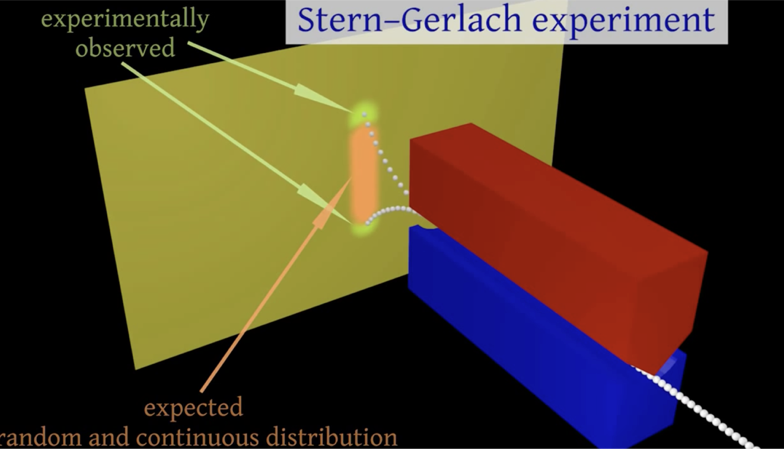
\includegraphics[scale=0.2]{img/sternGerlach3.png}
%In the Stern-Gerlach experiment (1922) a beam of silver atoms passed through an inhomogeneous magnetic field as shown in the sketch. The experiment was intended to test the space-quantization associated with the orbital angular momentum of atomic electrons, already described by the ``old quantum theory'' (Sommerfeld) which could be tested by making use of the fact that an orbiting electron will give rise to a magnetic moment proportional to the orbital angular momentum of the electron. 
%\column{0.5\textwidth}
%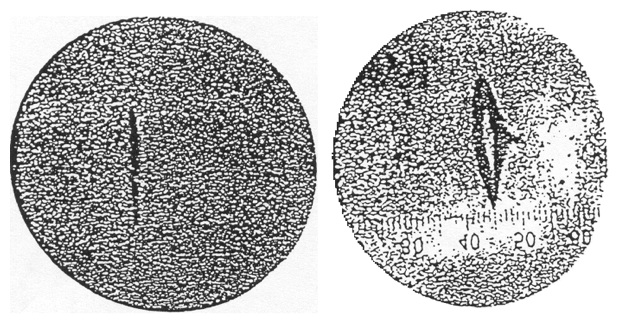
\includegraphics[scale=0.2]{img/sgSpots.jpg}
%The result of the experiment is shown  (picture from the original paper). There is an intensity minimum in the center of the pattern, and the separation of the beam into two components is clearly seen. This result seemed to confirm Sommerfeld's quantum-theoretical prediction of spatial quantization. 
%%Pauli, a notoriously skeptical physicist, remarked, ``Hopefully now even the incredulous Stern will be convinced about directional quantization'' (in a letter from Pauli to Gerlach 17 February 1922). 
%\end{columns}
%\end{frame}
%\begin{frame}
%
%\frametitle{Stern Gerlach experiment: Spin is real}
%
%There are 47 electrons surrounding the silver atom nucleus, of which 46 form a closed inner core of total angular momentum zero -- there is no orbital angular momentum, and the electrons with opposite spins pair off, so the total angular momentum is zero, and hence there is no magnetic moment due to the core. The one remaining electron also has zero orbital angular momentum, \alert{so the sole source of any magnetic moment is that due to the intrinsic spin of the electron.}
% 
%Thus, the experiment represents a direct measurement of one component of the spin of the electron, this component being determined by the direction of the magnetic field, here taken to be in the z direction.
%
%There are two possible values for $S_z$~ corresponding to the two spots on the observation screen, implying that $s = 1/2$. The allowed values for the $z$~component of the spin are:
%\[
%S_z = \pm \frac{1}{2}\hbar
%\]
%
%Of course there is nothing special about the direction $z$. Any component of the spin of an electron will have only two values. If $\vv{\bm{n}}$ is a unit vector specifying some arbitrary direction then:
%\[
%\vv{\bm{S}} \cdot \vv{\bm{n}} = \pm \frac{1}{2}\hbar
%\]
%\end{frame}
%
%\begin{frame}
%\frametitle{NRQM and Pauli matrices}
%
%In NRQM we define $\ket{\uparrow}$~to be the state with spin in the $+z$~direction and 
%$\ket{\downarrow}$~to be the state with spin in the $-z$~direction.
% 
%\[
%\ket{\uparrow} = \mqty(1\\0), \,\,\, \ket{\downarrow} = \mqty(0\\1)
%\]
%
%In the space spanned by $\ket{\uparrow}$~and $\ket{\downarrow}$~the angular momentum operator is represented by the Pauli matrices
%\[
%J_i =\frac{\sigma_i}{2}, \,\,\, (i=1,2,3, ~{\rm or}~x,y,z)
%\]
%which satisfy the commutation relation of angular momentum operators, 
%$[J_i, J_k] = i \epsilon_{ijk} J_k$. The square of the angular momentum operator $\va{J^2}$ is:
%\[
%\va{J^2} =J_1^2 + J_2^2 + J_2^2 = j(j+1)
%\]
%But then: 
%\[
%\frac{\va{\sigma^2}}{2} =(\frac{\sigma_1}{2})^2 + (\frac{\sigma_2}{2})^2 + (\frac{\sigma_3}{2})^2 
%= \frac{3}{4} = \frac{1}{2}(\frac{1}{2} + 1)
%\]
%$\va{\sigma}/2$~ is  a spin-1/2 representation of angular momentum.
%\end{frame}
